\documentclass[conference]{IEEEtran}
\IEEEoverridecommandlockouts
% The preceding line is only needed to identify funding in the first footnote. If that is unneeded, please comment it out.
\usepackage{balance}
\usepackage{booktabs}
\usepackage{cite}
\usepackage{amsmath,amssymb,amsfonts}
\usepackage{algorithm}
\usepackage{algpseudocode}
\usepackage{graphicx}
\usepackage{listings}
\usepackage{sourcecodepro}
\usepackage{textcomp}
\usepackage{xcolor}

\lstset{
  basicstyle=\footnotesize\ttfamily,
  frame=single,
  tabsize=2,
}

\lstset{
  emph={
    message, rpc, string, enum, bytes, service, returns
  },
  emphstyle=\textbf
}

\begin{document}

\title{Building Scalable Systems for Neural Architecture Search with RPC}

\author{\IEEEauthorblockN{Jeff Hajewski}
\IEEEauthorblockA{\textit{Department of Computer Science} \\
\textit{University of Iowa}\\
Iowa City, IA, USA\\
jeffrey-hajewski@uiowa.edu}
\and
\IEEEauthorblockN{Suely Oliveira}
\IEEEauthorblockA{\textit{Department of Computer Science} \\
\textit{University of Iowa}\\
Iowa City, IA, USA \\
suely-oliveira@uiowa.edu}
}

\maketitle

\begin{abstract}
  word word word word word word word word word word
  word word word word word word word word word word
  word word word word word word word word word word
  word word word word word word word word word word
  word word word word word word word word word word
  word word word word word word word word word word
  word word word word word word word word word word
  word word word word word word word word word word
  word word word word word word word word word word
  word word word word word word word word word word
\end{abstract}

\begin{IEEEkeywords}
distributed deep learning, neural architecture search, artificial intelligence
\end{IEEEkeywords}

\section{Introduction}
Building robust and scalable distributed applications is challenging --- getting
communications patterns correct, handling node failures, and allowing for
elastic compute resources (where compute nodes may join or leave the system
throughout the life of the application) all contribute to a high level of
complexity. These challenges are exacerbated for long-runnining applications
such as training large deep learning models or neural architecture search. Among
the many popular frameworks for distributed programming, MPI
\cite{Forum:1994:MMI:898758} combined with additional accelerator paradigms such
as OpenMP \cite{Dagum:1998:OIA:615255.615542}, OpenACC
\cite{Wienke:2012:OFE:2402420.2402522}, and CUDA
\cite{Nickolls:2008:SPP:1365490.1365500} is the common choice for
performance-critical numerical workloads. In the deep learning setting, MPI is
less popular with many favoring mutli-threading in combination with multiple
GPUs, and more recently experimenting with Kubernetes \cite{8094194,
  8672301}. The fault tolerance required for long-running model training (which
can last on the order of months in the industrial setting) makes MPI a poor
choice for the underlying communication infrastructure. These types of applications
benefit from communication frameworks that are robust to failure and allow
for elastic compute settings. Remote procedure calls (RPCs) meet these
criteria and provide better communication infrastructure for large-scale
deep learning worklaods over MPI, which either does not offer, or offers with
significant implementation overhead.

In this work we propose an RPC-based system for distributed deep learning. We
experiment with the proposed architecture in the domain of neural architecture
search (NAS), a computationally intensive problem that trains thousands of deep
neural networks in search of an optimal network architecture.  We use this
problem domain to illustrate four primary advantages to building a
computationally intensive distributed system using RPC:
\begin{itemize}
\item RPC's higher level of abstraction over MPI simplifies the process of
  building more complex systems and communication patterns.
\item The user can avoid lower-level message serialization and deserialization
  (e.g., buffer allocation and deallocation)
  through RPC coupled with frameworks such as Protocol Buffers or Thrift.
\item RPC systems don't require underlying software or resource managers --- a
  user can create an AWS instance and immediately run their RPC-based code.
\item RPC-based systems can offer elastic compute abilities, adding or removing
  nodes as needed without needing to stop or restart the system. This can be
  particularly useful when combined with an orchestration technology such as
  Kubernetes, Amazon Container Service, Azure Container Service, or Google
  Container Engine.
\end{itemize}

Our system consists of four separate pieces: a \emph{model} that directs the
search for a network architecture, a number of \emph{workers} that perform the
computational work of training and evaluating the network architectures, at
least one \emph{broker} that forms the data pipeline from model to workers, and
a \emph{nameserver} that simplifies the process of adding new brokers, workers,
and models to the system in addition to managing system metadata. Our system
also offers elastic compute resources, allowing an arbitrary number of workers
to join during high computational loads as well as allowing workers to leave the
system during periods of reduced computational load, decreasing the overall
available compute, without needing to restart or manual intervention.  The
system is fault-tolerant to the loss of workers or brokers and is highly
scalable due to the ability of the brokers to share work and compute
resources. Perhaps most importantly from a usability perspective, our system is
language agnostic. In our experiments, we use Python for our model and workers,
which we use to build and train deep neural networks via PyTorch
\cite{paszke2017automatic}, and use Go to build the data pipeline of brokers. We
use gRPC \cite{Wang:1993:GCC:155870.155881} to handle the generation of RPC
stubs, but could have just as easily used Apache Thrift \cite{Slee2007}, which
generates stubs in a larger range of languages such as Ocaml, Haskell, and Rust.

Although we are proposing RPC as an alternative to MPI, it is important to note
that we are not claiming RPC is superior to MPI in every problem domain. In the
domain of distributed deep learning, RPC offers many useful features. In other
domains, such as distributed linear algebra, MPI is probably a better choice due
to its built in ability to efficiently broadcast messages to nodes within a
system in a manner that takes advantage of the physical network architecture.

\section{Neural Architecture Search}
The goal of neural architecture search (NAS) is to find an optimal neural
network architecture for a given problem. Denote the training data as
$X_{\text{tr}}$ and $y_{\text{tr}}$, and a trained neural network as
$\Psi(\mathbf{x}; X_{\text{tr}}, y_{\text{tr}})$, then the problem
neural architecture search attempts to solve is given by
Equation~\eqref{eq:problem}.
\begin{equation}\label{eq:problem}
\Psi^* = \arg\min_{\Psi \in \mathcal{A}} L(X_{\text{val}}, y_{\text{val}}; \Psi(\mathbf{x}; X_{\text{tr}}, y_{\text{tr}}))
\end{equation}

where $X_{\text{val}}$ and $y_{\text{val}}$ are validation datasets and $L$
is a loss function. We use the negative log-likelihood loss function. The
space of neural network architectures is denoted $\mathcal{A}$ and is an
infinite dimensional space.

NAS is computationally intensive due to the cost of evaluating networks, which
involves both training and validating the network.  Although recent novel
approaches have dramatically reduced this cost
\cite{DBLP:journals/corr/abs-1708-05344, pmlr-v80-pham18a}, these techniques fix
certain elements of the design process, somewhat limiting the available
architectures. Despite the computationally intense nature of the NAS problem,
the task itself is trivially parallelizable across the network evaluations ---
two separate networks can be trained simultaneously before being evaluated
against eachother.

The two common approaches to NAS are reinforcement learning based approaches such
as \cite{45826, Kyriakides:2018:NAS:3200947.3208068, pmlr-v80-pham18a}, and
evolutionary approaches such as \cite{DBLP:journals/corr/abs-1711-00436,
  DBLP:journals/corr/MiikkulainenLMR17, DBLP:conf/icml/RealMSSSTLK17}. In our
experiments we focus on the evolutionary approach due to its simplicity in both
understanding and implementation.

\subsection{Evolutionary Neural Architecture Search}
We use a relatively simple approach to evolving neural network architectures in
that we only construct linear networks, rather than allow an arbitrary number of
incoming and outgoing connections for any given layer. The motivation behind
this is two-fold: it reduces the size of search space for the neural network
architecture and simplifies the implementation. Because the focus of this work
is the system architecture, rather than neural architecture search, we feel the
trade-off is reasonable.
% 
% \begin{figure}
%   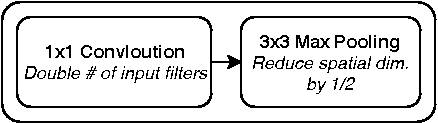
\includegraphics{img/reduction}
%   \caption{Reduction layer.}
%   \label{fig:reduction}
% \end{figure}

The problem domain we focus on is computer vision, so we restrict ourselves
to convolutional layers for the hidden layers. Repeated network modules
form the core network architecture. A single module is found via evolutionary
search and this module is repeated several times to build the network, as
shown in Figure~\ref{fig:sample-arch}.
Within a module, each convolutional layer uses zero padding to maintain the
spatial dimensions of the input while allowing filter size and depth to be
chosen through evolution. ReLU activation functions are inserted between
layers and after reductions.
We use the heuristic of doubling the number of filters
via a 1x1 convultional layer prior to reducing the spatial dimension by a
factor of two via a 2x2 max pooling layer with a stride of two.
The intuition behind this
technique is to control information loss across reduction layers. The spatial
reduction results in a 75\% loss in spatial information. Increasing the
number of filters by a factor of two increases the total information transfered
from the layer before the reduction layer to the layer immediately following
the reduction layer to at most 50\% instead of 25\%.

Module evolution proceeds by appending layers to the module or performing
crossover, where two networks are split at random positions and recombined
to form a new network. The maximum number of layers in a module is fixed
(by the user), and evolution can add either 3x3 or 5x5 2D convolutional
layers with filter depths of 16, 32, 64, or 128.

\begin{figure*}
  \centering
  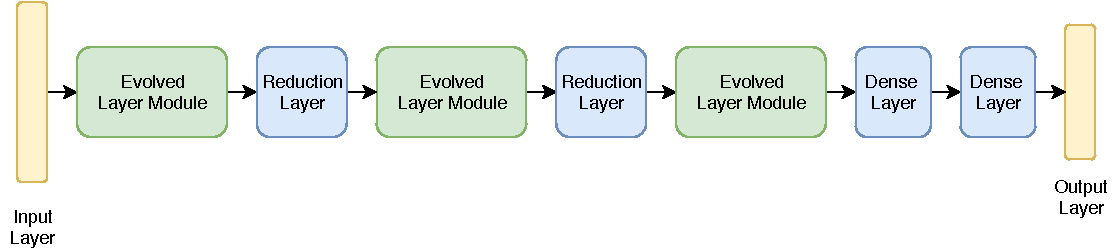
\includegraphics[width=.85\textwidth]{img/sample_arch}
  \caption{Example of a constructed network.}
  \label{fig:sample-arch}
\end{figure*}


\begin{algorithm}
  \caption{High-level outline of evolutionary algorithm.}\label{alg:evo-simple}
  \begin{algorithmic}[1]
    \Procedure{ProduceOffspring}{$N_1, N_2$}
    \If{$|N_1| \neq |N_2|$}
    \State $o_1\gets N_1.\texttt{mutate()}$
    \State $o_2 \gets N_2.\texttt{mutate()}$
    \State \textbf{return } $o_1, o_2$
    \EndIf
    \State $o \gets N_1.\texttt{crossover}(N_2)$
    \State $o.\texttt{mutate()}$
    \State \textbf{return } $o$
  \EndProcedure
  \Procedure{Mutate}{}
  \State \emph{// Possibly append layer}
  \If{$\texttt{sampleUniform(0, 1)} < \texttt{append\_p}$}
  \State \texttt{self.layers.append}(\texttt{randomLayer()})
  \EndIf
  \EndProcedure
  \end{algorithmic}
\end{algorithm}

\section{RPC-based Communication}
Remote Procedure Call (RPC) is a method of invoking a function on a remote
computer with a given set of arguments. Most RPC frameworks involve an interface
description language (IDL)
to define the RPC service (that is, the API available to the caller) and some
type of data serialization format. For example, gRPC uses Protocol Buffers (ProtoBufs)
\cite{Varda2008} as the serialization format for data sent across the network.
RPC offers a number of advantages for network communication. It is robust to
node failures or network partitions (the RPC invokation simply fails). The data
sent across the network is compactly represented, giving way to high bandwidth
and low latency communication. And lastly, the point-to-point communication allows for
diverse communication patterns and paradigms. RPC forms the network communication
infrastructure at Google \cite{van2017production}, Facebook \cite{Slee2007},
as well as Hadoop
\cite{Shvachko:2010:HDF:1913798.1914427, Lu:2013:HDH:2570457.2571128}.

Figure~\ref{fig:heartbeat} gives an example of a gRPC service
definition for a heartbeat service. The ProtoBuf compiler uses this definition
to generate server stubs and service clients in a number of languages (C++,
Java, Python, Go, etc.). The receiver of the RPC call must complete the server
stubs by implementing the defined interface. For example, in the heartbeat
service defined in Figure~\ref{fig:heartbeat}, the receiver of the heartbeat
message would implement a \texttt{SendHeartbeat} function whose body would
handle the logic of \emph{receiving} a heartbeat from another process,
such as updating a timestamp for the given process ID. The caller of
\texttt{SendHeartbeat} uses the generated Heartbeat service client to invoke
the heartbeat RPC and is only
responsible for constructing the request body, \texttt{HeartbeatMsg}.

\begin{figure}
  \begin{lstlisting}
service Heartbeat {
  rpc SendHeartbeat(Heartbeat) returns (HBResp) {}
}
message Heartbeat {
  string id = 1;
}
message HBResp {}
\end{lstlisting}
\caption{Example gRPC service definition of a heartbeat service.}
\label{fig:heartbeat}
\end{figure}

While the robustness to node failures and finer-grained point-to-point
communication capabilities of RPC are core to building resilient distributed
systems, the more powerful feature we capitalize on is the ability to build a
system that is agnostic to the type of data flowing through its
pipes. Figure~\ref{fig:data-agnostic} gives an example of constructing a
Protocol Buffer message type that can be used to transport arbitrary data types
through the system. Protocol Buffers (and similarly, Thrift messages) support
variable length byte arrays
\footnote{In practice these arrays are limited in size. The failure rate of the
  RPC system typically increases with the size of the messages.} This means the
user can send a serialized object stored in the \texttt{Task}'s
\texttt{task\_obj} field without having to modify the system.  A user can switch
between running models and tasks using Java to running models and tasks using
Python without modifying the data pipeline. In fact, the system can transport
and run these tasks (in both Java and Python) simultaneously. By encapsulating
the tasks (and results) as serialized objects stored as byte arrays, the entire
system can be data type agnostic.

\begin{figure}
  \begin{lstlisting}
message Task {
  string id = 1;
  enum type = 2; // or string type
  bytes task_obj = 3;
}
  \end{lstlisting}
  \caption{Example of a data agnostic message type.}\label{fig:data-agnostic}
\end{figure}

There is a slight catch. If information within the serialized object
is needed to properly schedule or transport the task/result to its
destination, this information will need to be added to the message
definition. This requires recompiling the message types and regenerating
the gRPC (or Thrift) stubs. This is a minor inconveninece, as incorporating
this new information into the system requires modifying the system
infrastructure.

A final advantage of using gRPC or Thrift to define the RPC API of the system is
the service definition itself acts as documentation on the flow of information
within the system. A user can look at these definitions and see how information
is meant to flow. Understanding the communication patterns of a system built
with a lower-level message passing framework such as MPI or $\varnothing$MQ requires
reading through the source code. This may not be an issue for simple MPI applications
where a majority of the communication logic is in a main run-loop, but for larger,
more complex projects this increases the cognitive load on the user.

\begin{figure}
  \begin{lstlisting}
service Task {
  // Called by a worker to request a task.
  rpc RequestTask(TaskRequest)
    returns (TaskResponse) {}
}
service Result {
  // Called by a worker to send a result
  // back to the broker.
  rpc SendResult(ResultMsg)
    returns (ResultResponse) {}
}
  \end{lstlisting}
  \caption{Example service definitions for tasks and results.}
  \label{fig:task-result-services}
\end{figure}

\subsection{RPC vs MPI}
From a performance perspective, some prior work \cite{rpc-perf} has found RPC to
provide lower latency and higher bandwidth for some tasks. That does not tell
the entire story. MPI comes with built-in complex communication primitives that
are capable of taking advantage the physical network architecture of the
cluster. Additionally, MPI is capable of bulk broadcasts to groups of nodes
using custom communicator definitions. These primitives save the programmer a
lot of overhead when building HPC applications. Settings such as large,
distributed matrix multiplications or iterative optimization algorithms are
particuarly well suited for MPI's communication primitives.

However, applications that benefit from specialized communication patterns or
that are different processes communicating asynchronously typically better
suited for RPC-based communication. Consider, for example, an application that
sends some amount of work to a number of worker nodes and waits for the work
to be completed, such as a distributed deep learning workload \cite{40565}. In the
synchronous setting, the entire system will only be as fast as its slowest node
and will cause idle resources as the faster nodes wait for the slowest node to
finish. In the asynchronous setting, the faster nodes can continue to process
additional work while the slower nodes work on their original tasks. MPI can
handle this type of a setting using the asynchronous APIs \texttt{mpi\_Isend}
and \texttt{mpi\_Irecv}; however, the MPI application logic will become increasingly
complex if the number and type of workers is dynamic. This is because MPI uses
process IDs for communication, requiring the user to use message routing logic
based on these IDs. When the communication numbers and patterns change, this
apporach can become difficult to modify whereas a more flexible approach such
as RPC can handle the changes with no change to application logic (e.g., simply
start more worker processes).

One short-coming of RPC is message size limitations. This can be particularly
troublesome in distributed machine learning settings where highly parameterized
models such as deep neural networks are sent across the network. The solution
is to send a representation of the model, rather than the model itself, across
the network. The advantage of this approach is reduced network bandwidth
utilization. The disadvantage of course is the loss of trained models at the
worker nodes. In practice, this may not be a major issue as final model
architectures are typically trained in a specialized manner (e.g., for a large
number of epochs). Additionally, models can be saved to a distributed filesystem
such as HDFS.

Of course, MPI does offer asynchronous communication, but it is not as flexible
as that of RPC-based systems. In an asynchronous setting there are usually
classes of nodes whose behavior are class-dependent. In the system we propose,
there are four classes of processes: the model, the broker, the nameserver, and
the worker. It is conceptually simpler to think of these as four different
services and build each of them separately using a service-oriented
architecture, rather than a single program that determines its behavior based on
its assigned communicator rank (as done in MPI).

An interesting advantage of RPC is the ability to take advantage of a container
orchestration system such as Kubernetes \cite{43826} to ensure a specified
number of worker nodes remain available. If a worker node goes down, or the
desired number of worker nodes increases, Kubernetes restores the system to
the desired state automatically. This is only possible because RPC allows us to
create stateless communication channels that do not require a persistent connection
between communicating nodes. While this may seem excessive for a small collection
of nodes, the ability to have Kubernetes manage system state within a large
system can be quite valuable in a production system.

One particularly unique aspect of the domain of neural architecture search is
that it does not require low-latency communication. Each neural network can take
anywhere from minutes to hours to train, which means the frequency of
task and corresponding result messages is fairly low. One prior work
\cite{DBLP:conf/icml/RealMSSSTLK17} even used a shared filesystem to communicate
between a model and the worker nodes. The long time interval between sending the
task to the worker and receiving the result from the same worker means a single
server could handle a potentially large number of connections with workers,
certainly on the order of hundreds and possibly even thousands.
% Anecdotally, we
% found that a laptop with an Intel 4.2GHz i7 processor was able to handle over 200
% connections of a heartbeat request and response service where heartbeats are sent
% every second, similar to that depicted in Figure~\ref{fig:heartbeat}.

\section{System Architecture}
As previously mentioned, our system consists of four different components.
Figure~\ref{fig:sys-arch} shows an overview of the system architecture.  A model
is a problem specific implementation that controls what is sent to the system
for evaluation and handles the result it receives. The brokers form the data
pipeline of the system, moving work from the models to the available workers.
Workers form the other
customizable part of the system because they need to know how to perform their
assigned work.  Lastly, the nameserver maps known brokers to their network
address -- this is useful for connecting to brokers, such as a model connecting
to a broker, a broker connecting to a broker (for broker-broker peering), or a
worker connecting to a broker. The following sections will detail each
components functionality individual and within the system as a whole.

\begin{figure}
  \centering
  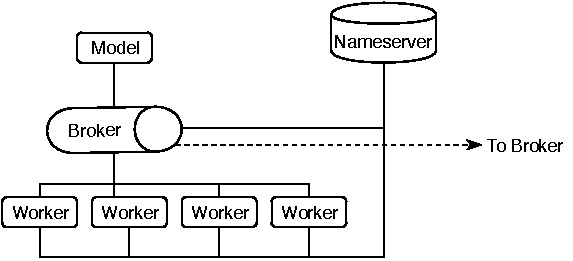
\includegraphics[width=.85\columnwidth]{img/system-arch.pdf}
  \caption{Diagram of system architecture.}
  \label{fig:sys-arch}
\end{figure}

\subsection{Model}
The model is the problem-specific, user-defined logic that determines what work
should be performed next and how the results of previously assigned work should
be processed. The only requirement of the model is that is uses a broker client
stub (generated by gRPC) to push work to the system and implements the result
service interface, depicted in Figure~\ref{fig:task-result-services}, to allow
the broker to push results back to the model.

The model needs to track outstanding tasks that have been sent to the broker.
While the system is fault-tolerant for most brokers and all workers, if the
broker the model is sending work to fails, the work the model is waiting to
receive will be lost and the model will need to resend to a new broker. The
simplest approach to handle this state is via a heartbeat.

\begin{figure}
  \centering
  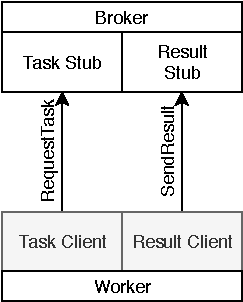
\includegraphics{img/broker_worker}
  \caption{Communication pattern between a worker and broker.}
  \label{fig:worker-broker}
\end{figure}

\subsection{Worker}
Workers are the other user-defined and implemented portion of the system. While
a single worker implementation can work for multiple model implementations,
there is no general worker implementation that will work across all languages
and models.

\begin{figure}
  \begin{lstlisting}[language=python]
class BaseTask:
  def run(self):
    raise NotImplementedError()

class Worker:
  def process_task(self, task):
    result = task.run()
    self.broker_client.send_result(result)
  \end{lstlisting}
  \caption{Example Task API in Python.}\label{fig:python-api}
\end{figure}

Using an API similar to that shown in Figure~\ref{fig:python-api}, one can use
the same worker implementation for any task that inherits from the
\texttt{BaseTask} class. This means the same worker applications can be used
from any problem that designs its tasks to inherit from \texttt{BaseTask},
regardless of whether that problem is training and evaluating neural networks
or factoring large numbers. As long as the task implements a \texttt{run()} method,
the worker can execute the task without a change in logic.

Figure~\ref{fig:worker-broker} shows the communication pattern between the
broker and a worker. There are two interesting aspects of this diagram: all
communication starts at the worker and there is no heartbeat exchange between
the worker and the broker. Both of these details are what allow the system to
treat workers as ephemeral compute resources. This means an arbitrary number of
workers can join and leave the system without the system knowing or caring. The
downside to this approach is it requires a little extra bookkeeping at the
broker. The broker needs to track what tasks are outstanding and decide if they
should be moved back in to the work queue.

\subsection{Broker}
Brokers form the data pipeline of our system. Work is sent from a model to a
broker, which in turn sends the work to a free worker or to another broker via
peering and returns the result to
the original model. At its core, a broker is essentially just a process with a
owned task queue, a helper task queue (tasks received from other brokers
via peering), a
processing queue, and a results queue. Work in the owned task queue is work that
was sent from a model directly to the broker -- this is the work that will be
lost if the broker crashes. Work in the helper task queue is work that has been
sent from other brokers that the respective broker has agreed to help with. If
the broker crashes, this work will \emph{not} be lost as the other brokers will
see the failure and can recover the task from their processing queue. The
processing queue stores tasks that have been sent to workers or other
brokers. When a result is received from a worker or another broker, the
corresponding ID will be removed from the processing queue and the result will
be added to the result queue. The broker pulls tasks from the result queue and
sends the result to its owner, which may be a model or another broker.

\begin{figure}
  \centering
  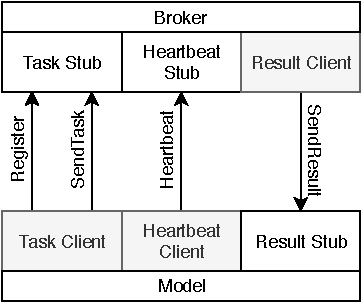
\includegraphics{img/model_broker}
  \caption{Communication pattern between the broker and
    model.}\label{fig:broker-model}
\end{figure}

\subsection{Nameserver}
The nameserver simplifies bookkeeping when starting new broker instances.
Rather than forcing the user to specify which brokers a newly started broker
should link up with, the nameserver stores and shares that information with all
registered brokers. During start-up, each broker registers with the nameserver
and begins sending heartbeat messages. The nameserver tracks which brokers have
sent heartbeats recently (via a user-modifiable timeout setting) and drops
brokers that have timed-out. If a broker sends a heartbeat \emph{after} the
nameserver has dropped the connection, the nameserver responds by telling the
broker it must re-register with the nameserver.

The nameserver simplifies broker-broker peering by providing a central location
where brokers can request addresses of other brokers. It also provides a metadata
store for the system, which is important in multi-GPU scenarios. A worker running
on a server with multiple GPUs needs information about what GPU to use. Storing
this metadata on the nameserver allows the nameserver to manage GPU resources,
rather than requiring the user to specify the GPU ID for every worker that is
running, which is not scalable for hundreds or thousands of workers.

% 
% Care must be taken with the nameserver as this is the single point of failure
% within the system. Although the system can continue to function without a
% nameserver, new brokers will be unable to join. This means eventually the system
% will fail as brokers leave the system (e.g., power outage, hardware failure,
% etc.).  The simple solution is to use an orchestration system such as Kubernetes
% to make sure there is always at least one nameserver running. Because the
% nameserver can force brokers to re-register, restoring a failed nameserver
% simply forces all incoming heartbeat requests to re-register and thus restoring
% the state of the nameserver broker registry prior to the crash. This mechanism
% greatly simplifies the implementation of the nameserver. The only state that
% must persist between crashes of the nameserver is that of the next available
% broker ID. If the nameserver does not persist this to some type of durable
% medium (e.g., HDFS \cite{Shvachko:2010:HDF:1913798.1914427}) then it is possible
% for multiple brokers to receive the same broker ID.
% 
\begin{figure}
  \centering
  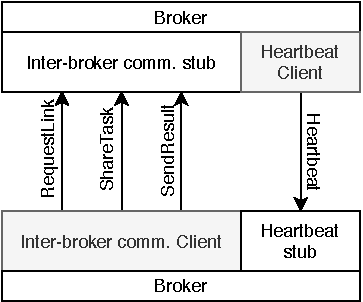
\includegraphics{img/broker_broker}
  \caption{Communication pattern for broker-broker communication.}
  \label{fig:broker-broker}
\end{figure}

\section{Discussion}
The goal of our experiments is to explore the scalability and robustness
of a system built using RPCs for communication to perform a long-running,
computationally intensive task. We use the CIFAR-10 \cite{cifar10-data}
dataset because it is small enough to allow us to train reasonably
performing neural networks in a short amount of time when compared with
datasets such as CIFAR-100 \cite{cifar100-data} or ImageNet \cite{imagenet_cvpr09}.
All experiments were run on Amazon's
AWS EC2 platform using \texttt{p2.8xlarge} instances consisting of 8
Nvidia K80 GPUs. The first run on a single GPU sets the baseline
number of models evaluated per generation. The successive experiments
analyze how this value changes with the addition of worker nodes as well
as how the system reacts to losing worker nodes.
\subsection{Scalability}
Figure~\ref{fig:scale} shows the scaling results, which are computed as the
geometric mean across five generations of neural network evolution. Five
generations was chosen primarily due to resource limits. The relative scaling
decreases as the number of workers (GPUs) increases primarily due to an
increase in the rate of idle workers and worker failures. More workers
means the workers are able to evaluate the candidate networks (composing a
generation) in a shorter total amount of time; however, not all networks
take the same amount of time to evaluate, leading some workers to remain
idle while waiting for other workers to finish.

The other issue impacting the scalability of the system is worker
failures. With larger worker counts the system encountered larger models
sooner and some of these models exhausted the GPU's memory. We also
suspect there was a GPU memory leak in our PyTorch code but were unable
to find the root cause. We manually restarted failed workers; however,
we were not constantly monitoring worker status and as a result the higher
worker runs were sometimes running several workers down. This is a great
example of a scenario where an orchestration system such as Kubernetes,
Apache Mesos, or similar offerings from AWS, GCP, and Microsoft Azure.
The ability to automatically restart failed workers would have improved
the overall scalability results.

\begin{figure}
  \centering
  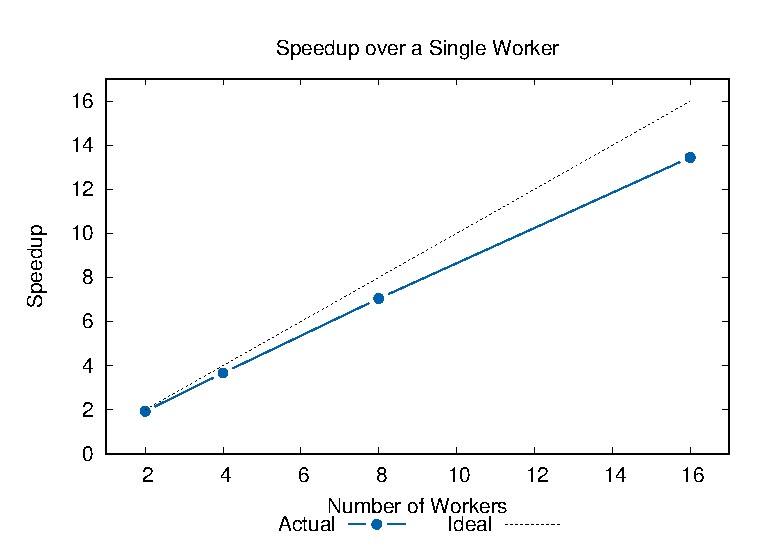
\includegraphics[width=\columnwidth]{result/output/rates}
  \caption{Speedup as a function of the number of workers over a single worker,
    calculated as the geometric mean across 5 generations.}
  \label{fig:scale}
\end{figure}

\begin{table}
  \centering
  \caption{Failures over time}
  \label{tab:failures}
  \begin{tabular}{cc}\toprule
    \textbf{Workers} & \textbf{\# Failures}\\\midrule
    1 & 0\\
    2 & 0\\
    4 & 2\\
    8 & 8\\
    16 & 13\\\bottomrule
  \end{tabular}
\end{table}
\subsection{Node Failures}
Table~\ref{tab:failures} raises another interesting issue with respsect
to keep workers busy evaluating network architectures. Handling a failed
worker is relatively simple: the model tracks how many networks were
sent for evaluation and pops the same number of results off the result
queue, which blocks for a specified timeout. We new from experience the
average network took about two minutes to train, so we set the timeout to
five minutes times the number of models sent for evaluation. This works
but is incredibly inefficient for the workers who are sitting idle when
they could have been evaluating two additional networks each. Idle servers
are expensive, especially when running specialized hardware on services
such as AWS or GCP.

One possible solution is to switch from a generational approach to evolution
and use a competition-based approach. In the competition approach the model
waits for the result queue to have two results and drops the network architecture
that has a worse fitness (validation accuracy, in this case).

\subsection{Found Architectures}
Figure~\ref{fig:best} shows the best found architecture after five generations.
Somewhat unsurprisingly, there were many other architectures that performed
similarly to this architecture. One characteristic common in all of the high
performing architectures is a high number of filters in the first layer of
the module. This characteristic is not a sufficient condition for strong
performance. Some networks with a very large filter depth in the first layer
performed poorly, possibly due to over-fitting, while others with an average
filter depth but small filter spatial dimensions also performed poorly.

These results illustrate the challenge of designing effective neural
networks---seemingly similar networks may have dramatically different
performances. Consider Figure~\ref{fig:good-bad}, which shows to neural
networks with similar architectures. The network on the left had a validation
accuracy of 72.6\% (that is, it got about three out of every four classifications
correct on previously unseen data) while the network on the right had a
validation accuracy of 10.1\%.

\begin{figure}
  \centering
  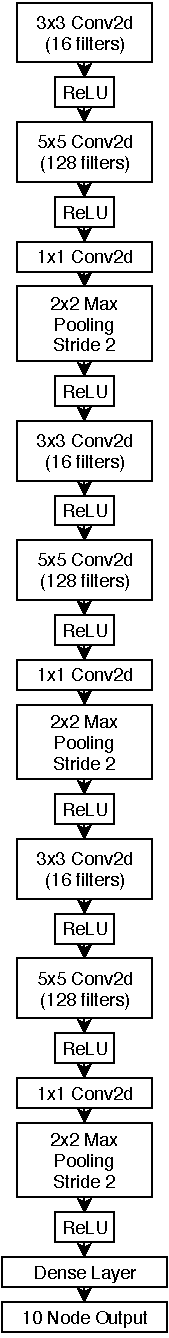
\includegraphics[height=.45\textheight]{img/best-model}
  \caption{Architecture of best found network.}
  \label{fig:best}
\end{figure}

\begin{figure}
  \centering
  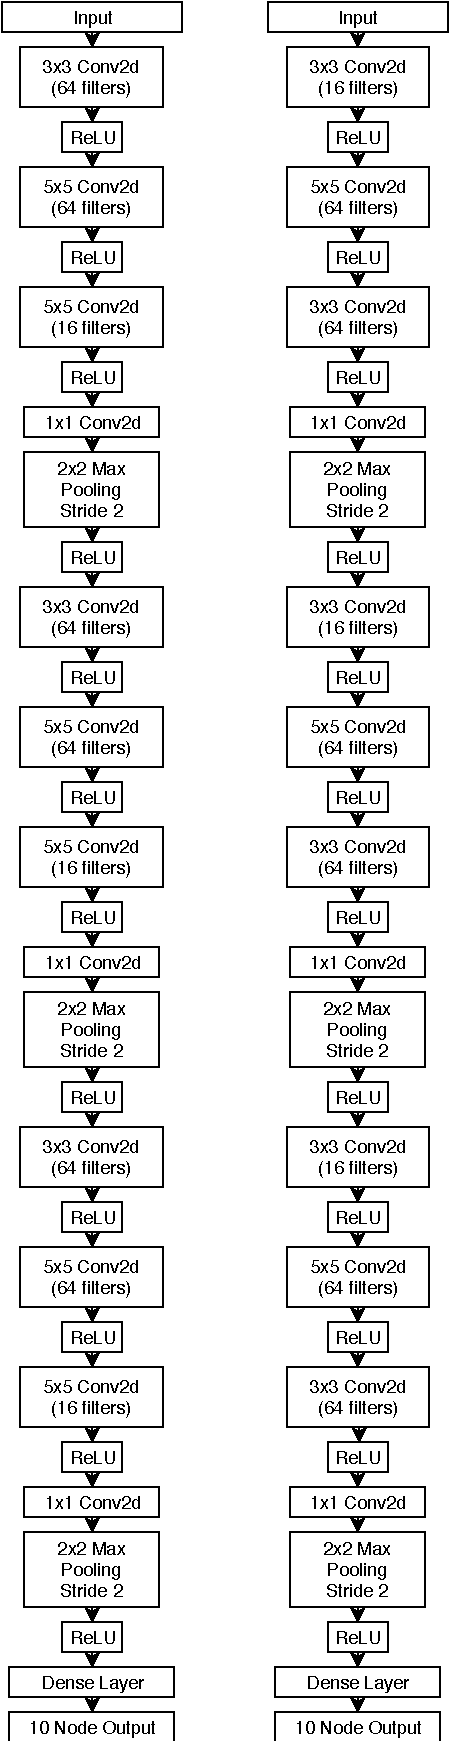
\includegraphics[height=.45\textheight]{img/good-bad}
  \caption{(left) Architecture of a network performing close to the
    best found architecture. (right) Architecture of a network performing
    at the bottom of all found networks.}
  \label{fig:good-bad}
\end{figure}

\section{Related Work}
The idea of a brokered message queue is not new. RabbitMQ [CITE] is a general
purpose message broker that supports the same functionality demonstrated
in this paper, but messages are delivered based on a routing key, rather than
the first available worker. Similar to the RPC message definitions used in
this work, RabbitMQ uses a collection of bytes as the message body. For
streaming data, Apache Kafka \cite{kafka} is a good choice. Kafka is requires a
ZooKeeper \cite{Hunt:2010:ZWC:1855840.1855851} instance and is generally
more complex to setup and run.
Both RabbitMQ and Kafka are robust to failures. At the other end of the
spectrum, $\varnothing$MQ is a low-level messaging library that can be used
to build a performant, brokered messaging system similar to the one described
in this paper.

A natural question at this point in the work is why we would bother building our
own brokered system when there are industrial strength alternatives
available. These message passing systems\footnote{We use this as a generic term,
  since Kafka is not really a message queue.} stricly deal with sending and
delivering messages in a scalable and robust manner. Our broker does more than
simply relay messages---the broker is determining retry logic, hadling lost
tasks, [ADD OTHER STUFF].

Tensorflow \cite{tensorflow2015-whitepaper} offers some distributed training
facilities. Other work such as Horovod \cite{DBLP:journals/corr/abs-1802-05799}
has improved upon Tensorflow's built-in distributed training facilities. Work
has also been done on training deep learning models using MPI
\cite{pmlr-v28-coates13, DBLP:journals/corr/VishnuSD16}. However, all of these
works suffer from fault tolerance of workers and elastic compute
environments. Additionally, they require that MPI is installed on the cluster,
which is not an issue if the software is running on a University research
cluster or at a national lab, but requires the user to setup the underlying MPI
installation if run on a provisioned AWS, GCP, or Azure cluster.

MXNet \cite{DBLP:journals/corr/ChenLLLWWXXZZ15} introduces a declarative language
used to build a computation graph, which is then optimized and evaluated by the
MXNet engine, similar to Tensorflow pre-2.0. [NEEDS ADDITIONAL WORK]

Much of the previous work on neural architecture search uses some form of a
distributed architecture consisting of a model, (possible) a coordinator, and workers. The
coordinator handles assignment of work to the workers. While many of these works
don't detail the specifics of their system, we reviewed some of the available
code on Github. A popular paradigm is using Python's \texttt{multiprocessing}
module to run multiple models on a multi-GPU machine. These GPUs are fed from a
thread-safe queue. PyTorch offers a data parallel module that handles this
functionality  but currently struggles to fully utilize all available GPUs in
settings with 8+ GPUs, per the PyTorch documentation.Tensorflow provides similar
functionality for distributed training but instead relies on gRPC.

A number of prior works use MPI in conjunction with deep learning libraries
taking a data parallel approach \cite{Awan:2016:ELM:2966884.2966912,
  Awan:2017:SCM:3018743.3018769}. This is familiar to other work that takes
advantage of multithreading (such as Python's \texttt{multiprocessing} module)
but utilizes much larger systems. Awan et. al.
\cite{Awan:2018:OBD:3236367.3236381} build a model parallel system using
MPI, relying on MPI's efficient communication primitives to avoid excessive
blocking when cross-node dependencies. Unfortunately, all of these works
require MPI on the system they are running, which adds another dependency
to the software stack. These works also are unable to utilize newly available
resources without restarting the running process.

Others \cite{journals/corr/MoritzNSJ15, journals/corr/KimPJY16} use Spark
\cite{Zaharia:2016:ASU:3013530.2934664} to
train deep learning neural networks. Spark \emph{can} handle the addition or loss
of compute nodes, is robust to node failures (via HDFS) but struggles with
iterative algorithms. Both of these works use Spark to distribute Caffe
\cite{Jia:2014:CCA:2647868.2654889} models to GPU compute nodes
and implement asynchronous SGD. The main issue with Spark in this context
is that either the user must create a wrapper for the model in Scala or
use PySpark. Using PySpark is relatively simple, as long as your model is
written in Python. If your model is written in something other than Python
such as C++, then you must decide if its better to create a wrapper in Scala
(if you know Scala) or a Swig interface and call it from Python. Both of
these options seem more complex than implementing a server stub to send
models and using a pre-generated client to request models to train as well
as report the results.

Implementing algorithms that are iterative in nature in Spark poses another
issue. Spark does not handle iterative-style algorithms particularly well,
primarily due to the shuffle-stage of MapReduce (since Spark is built on
top of Hadoop).

\section{Conclusion}
One unexplored avenue of potential future work is reusing the discarded
neural network architectures in an ensemble. Much of the NAS literature
finishes the search with the best found architecture---it would be interesting
to explore a comparison between the best architecture and an ensemble of
architectures taking into account communication overhead and voting required
by the ensemble.

It can be tempting to think of system design as an all-or-nothing
decision---either build a system with MPI or build a system using RPCs. An
interesting avenue for future work is combining the two. Consider a workload
whose core unit of work is amenable to an MPI-based system but the individual
units of work are independent of eachother with the exception of possible
boundary interactions. A combination of RPC and MPI communication might be
ideal---using MPI within a single cluster to complete individual units of work
and RPC to communicate between clusters. In this way, individual clusters become
the workers of the system and can join and leave at will, while the broker
backbone manages sending tasks to the individual clusters and returning their
results to the model.
\balance
\bibliographystyle{abbrv}
\bibliography{/home/jhaj/research/bibliographies/bdl,
  /home/jhaj/research/bibliographies/comps_plan}


\end{document}
